\documentclass[12pt]{article}
\usepackage{longtable}
\usepackage{enumitem}
\usepackage{graphicx}
\graphicspath{ {./images/} }
\def\arraystretch{1.2}%
\usepackage[a4paper,
	bindingoffset=0.2in,%
        left=1.2in,
        right=1.2in,
        top=1.2in,
        bottom=0.5in,%
        footskip=.25in]{geometry}
\usepackage[utf8]{inputenc}
\usepackage{xltxtra,fontspec,xunicode}
\setromanfont[Numbers=Uppercase]{Inter}
\defaultfontfeatures{Scale=MatchLowercase}

\newenvironment{packed_enum}{
\begin{enumerate}[leftmargin=15pt, itemsep=0pt, parsep=0pt, font=\small]
  \setlength{\itemsep}{0pt}
  \setlength{\parskip}{0pt}
  \setlength{\parsep}{0pt}
}{\end{enumerate}}

\newenvironment{packed_enum_roman}{
\begin{enumerate}[I, leftmargin=15pt,  font=\small]
  \setlength{\itemsep}{0pt}
  \setlength{\parskip}{0pt}
  \setlength{\parsep}{0pt}
}{\end{enumerate}}

\newenvironment{packed_enum_alpha}{
\begin{enumerate}[leftmargin=15pt, label=\alph*., font=\small]
  \setlength{\itemsep}{0pt}
  \setlength{\parskip}{0pt}
  \setlength{\parsep}{0pt}
}{\end{enumerate}}

\newenvironment{packed_item}{
\begin{itemize}
  \setlength{\itemsep}{0.1pt}
  \setlength{\parskip}{0pt}
  \setlength{\parsep}{0pt}
}{\end{itemize}}

{
    \fontfamily{lmss}\selectfont 

    %opening
    \title{
        Defining Use Cases \\ 
        \small Team 4
    }

    \author{
        Thomas Ripp
        \and 
        Joseph Mirabile
        \and 
        Jose Cruz
    }

    \date{
        Stevens Institute of Technology \\
        \small\today
    } 

    \begin{document}
    \maketitle
    \tableofcontents
    \pagebreak
}
\section{Use Case Template}

    \begin{longtable}{| p{.20\textwidth} | p{.80\textwidth} |} 
    \hline
     Item & Content \\ 
     \hline
     ID & UC001 \\  
     \hline
     Name & Check-out    \\ 
     \hline
     Actors & \begin{packed_item}
        \small{
        \item Customer
        \item Cashier
        \item Payment Provider}
    \end{packed_item}    \\ 
    \hline
    Data & \begin{packed_item}
        \small{
            \item POS DB
            \item Payment Provider Service
        }
    \end{packed_item}    \\ 
    \hline
    Stimulus & Customer touch the screen and starts a checkout session\\ 
    \hline
    Response & The customer gets a receipt for the checkout session    \\ 
    \hline
    Comments & \begin{packed_item}
        \small{
            \item The costumer has enough funds to pay for the invoice
            \item All the system peripherals are working
            \item The payment provider is online
            \item The connection between the store and the payment 
            provider is working
            \item All the items have their own unique barcode
            \item The screen is a touch screen and is working
            \item The POS have enough cash to give back change
            \item The POS system has a working connection with the POS DB
        }
    \end{packed_item} \\ 
    \hline
     Description & \begin{packed_enum}
        \begin{footnotesize}
            \item The costumer starts a checkout session 
            \item The system goes from idle mode to regular mode
            \item The costumer scans the barcode of the item
            \item The system checks if the barcode exists in the POS system, 
            if the item doesn’t exist, it displays an error that 
            item is not found and goes to step 3.
            \begin{packed_enum_alpha}
                \item The customer could reach out to the cashier which can 
                determine if there is an issue with the barcode and replace it.
            \end{packed_enum_alpha}
            \item The system add the item to the bill
            \begin{packed_enum_alpha}
                \item The cashier could remove an item from the bill if the 
                customer request it
            \end{packed_enum_alpha}
            \item The costumer repeats from step 3 until all the items 
            are added to the bill
            \item The costumer sends a signal to the POS system that 
            he is ready to pay
            \begin{packed_enum_alpha}
                \item The system calculates the subtotal and taxes
                \item The customer selects “Pay in cash”
                \begin{packed_enum}
                    \item The system enables the peripherals to accept cash
                    \item The costumer puts the dollars and cents for the total 
                    amount of the order
                    \item The costumer confirm the amount
                    \begin{packed_enum}
                        \item If the customer overpays the system will dispense 
                        the change
                        \item If the customer underpay the system will prompt a 
                        message to the user that it needs to put more money and 
                        the system will repeat from step 7.b.i but the amount is 
                        going to be the missing amount
                    \end{packed_enum}
                \end{packed_enum}
                \item The customer selects "Pays with credit / debit card"
                \begin{packed_enum}
                    \item The system sends a signal that activates the payment 
                    terminal
                    \item The payment terminal sends a message so the user 
                    inserts the card
                    \item The costumer insert the card
                    \item The terminal reads the card
                    \begin{packed_item}
                        \item If is invalid, the payment terminal display an 
                        error message to the user
                    \end{packed_item}
                    \item The terminal connects to the payment provider service 
                    and make a charge
                    \begin{packed_enum}
                        \item If the user doesn't have enough funds it will 
                        display an error message to the user and will send a 
                        signal to the POS system that the transfer was 
                        a failure.
                        \item The system will return to Step 7.a.
                    \end{packed_enum}
                    \item The terminal sends a signal to the POS System that the 
                    transfer was successful and also display a message 
                    to the user
                \end{packed_enum}
            \end{packed_enum_alpha}
            \item The systems prompts the user if they would like the receipt
            \begin{packed_enum_alpha}
                \item If the costumer select yes, the costumer sends a signal 
                to the system to print the receipt
                \item If the customer selects no, the system goes to step 9
            \end{packed_enum_alpha}
            \item The system goes to idle mode
        \end{footnotesize}
    \end{packed_enum}    \\ 
     \hline
    \end{longtable}
\pagebreak

\section{Use Case Diagram}
\begin{center}
    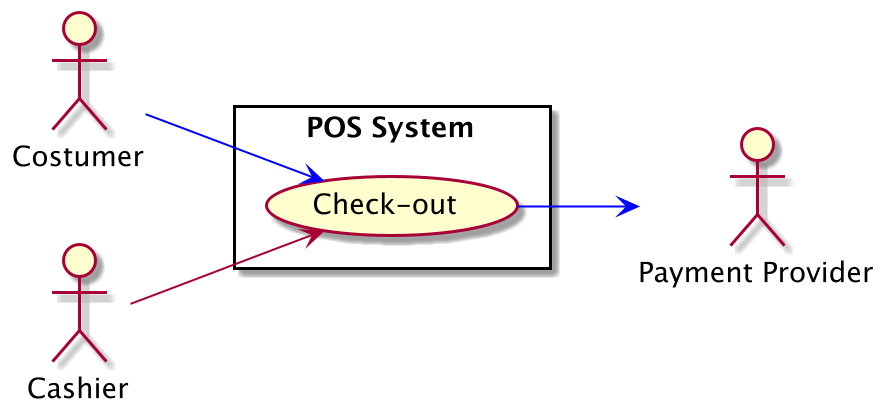
\includegraphics[scale=0.53]{diagram.png}
\end{center}
\pagebreak

\section{User Stories}
\subsection{Costumer}
    \begin{itemize}
        \item As a customer, I want to pay with credit card because 
        i don’t want to carry cash and i want the credit 
        card rewards (Step 7.c)
        \item As a customer, I want to pay with debit card because i don’t 
        want to carry cash and also i don’t want to spend 
        more than i have available (Step 7.c)
        \item As a customer, I do not want to wait in long lines to checkout.
        \item As a customer, I want to pay in cash so i don’t get in 
        debt by using credit cards (Step 7.b)
        \item As a customer, I would want the system to be able to apply any 
        coupons I have or any current discounts on any of my items 
        so I can save as much money as possible.
        \item As a customer, I would want the system to accurately 
        calculate my owed change so that I don’t overpay. (Step 7.a)
    \end{itemize}
\subsection{Cashier}
\begin{itemize}
    \item As a cashier, I want to be able to override items in 
    the order. (Step 5.a)
\end{itemize}
\end{document}